\documentclass[11pt,a4paper]{ltjsarticle}  % 日本語用クラス
\usepackage{luatexja}  % LuaLaTeX用日本語パッケージ
\usepackage{geometry}
\usepackage{listings}
\usepackage{adjustbox} % 図をページ内に自動フィット
\usepackage{xcolor}
\usepackage{hyperref}
\usepackage{tcolorbox}
\usepackage{enumitem}
\usepackage{here}
\usepackage{tikz}
\usetikzlibrary{backgrounds}
\usetikzlibrary{arrows.meta,positioning,fit,calc,shadows.blur}
\usepackage{graphicx}
\usepackage{fancyhdr}
\usepackage{amsmath}
\usepackage{longtable}

% 代替案: pLaTeX/upLaTeXを使う場合は以下を使用
% \documentclass[11pt,a4paper,dvipdfmx]{jsarticle}
% \usepackage[utf8]{inputenc}

\geometry{margin=2.5cm}

% ===================== 統一 listings スタイル =====================
\definecolor{codebg}{RGB}{247,247,247}

% bashStyle
\lstdefinestyle{bash}{
  language=bash,
  basicstyle=\ttfamily\footnotesize,
  breaklines=true,
  showstringspaces=false,
  frame=single,
  framerule=0.2pt,
  rulecolor=\color{black!25},
  backgroundcolor=\color{codebg},
  columns=fullflexible,
  aboveskip=6pt,
  belowskip=6pt,
  numbers=none
}

\lstdefinestyle{bashStyle}{
  language=bash,
  basicstyle=\ttfamily\footnotesize,
  breaklines=true,
  showstringspaces=false,
  frame=single,
  framerule=0.2pt,
  rulecolor=\color{black!25},
  backgroundcolor=\color{codebg},
  columns=fullflexible,
  aboveskip=6pt,
  belowskip=6pt,
  numbers=none
}

% pythonStyle
\lstdefinestyle{pythonStyle}{
  language=Python,
  basicstyle=\ttfamily\footnotesize,
  breaklines=true,
  showstringspaces=false,
  frame=single,
  framerule=0.2pt,
  rulecolor=\color{black!25},
  backgroundcolor=\color{codebg},
  columns=fullflexible,
  aboveskip=6pt,
  belowskip=6pt,
  numbers=none
}

% json
\lstdefinelanguage{json}{
  morestring=[b]",
  showstringspaces=false,
}
\lstdefinestyle{json}{
  language=json,
  basicstyle=\ttfamily\footnotesize,
  breaklines=true,
  showstringspaces=false,
  frame=single,
  framerule=0.2pt,
  rulecolor=\color{black!25},
  backgroundcolor=\color{codebg},
  columns=fullflexible,
  aboveskip=6pt,
  belowskip=6pt,
  numbers=none
}

% JavaScript
\lstdefinelanguage{JavaScript}{
  keywords={const,let,var,function,async,await,try,catch,throw,if,else,for,while,return,class,extends,new,this,null,true,false},
  morecomment=[l]{//}, morecomment=[s]{/*}{*/},
  morestring=[b]', morestring=[b]", morestring=[b]`,
  sensitive=true
}
\lstdefinestyle{javascriptStyle}{
  language=JavaScript,
  basicstyle=\ttfamily\footnotesize,
  breaklines=true,
  showstringspaces=false,
  frame=single,
  framerule=0.2pt,
  rulecolor=\color{black!25},
  backgroundcolor=\color{codebg},
  columns=fullflexible,
  aboveskip=6pt,
  belowskip=6pt,
  numbers=none
}

% ================================================================

% ===============================================================
% ヘッダー設定
\pagestyle{fancy}
\fancyhf{}
\rhead{OrdinalX API実践ガイド}
\lhead{\leftmark}
\cfoot{\thepage}

\title{OrdinalX (Better Wallet) API\\実践ガイド}
\author{Technical Documentation}
\date{\today}

\begin{document}

\maketitle
\tableofcontents
\newpage

\section{はじめに}

\subsection{このドキュメントについて}
このドキュメントは、\textbf{OrdinalX (Better Wallet) API}を実際に使用する開発者向けの実践的なガイドです。
Swagger仕様書の内容をより分かりやすく整理し、実装時の注意点やコツを含めて解説しています。

\subsection{OrdinalXとは}
\textbf{OrdinalX}は、BSV (Bitcoin SV) ブロックチェーン上でNFT(Ordinals)やBSVの送受信を管理するウォレットAPIサービスです。
以下の主要機能を提供しています:

\begin{itemize}
    \item BSVの送受信(Paymail対応)
    \item NFT(Ordinals)の作成・送信・管理
    \item ユーザー認証とウォレット管理
    \item トランザクション履歴の追跡
\end{itemize}

\subsection{API基本情報}
\begin{itemize}
    \item \textbf{ベースURL}: サーバごとに発行(本ドキュメントでは\url{https://akematsu.yenpoint.jp/})
    \item \textbf{認証方式}: JWT Bearer Token
    \item \textbf{プロトコル}: HTTPS
    \item \textbf{レスポンス形式}: JSON
\end{itemize}

\begin{tcolorbox}[colback=yellow!10,colframe=orange!50!black,title=重要な注意事項]
OrdinalXは1satoshiでのNFT(1SatOrdinals)作成に対応しています。これはBSVの最小単位である1satoshiにデータを刻むという革新的な技術です。
\end{tcolorbox}

\section{クイックスタート}

\subsection{基本的な使用フロー}

\begin{enumerate}
    \item \textbf{ユーザー登録} - \texttt{/api/v1/auth/sign-up}
    \item \textbf{ログイン} - \texttt{/api/v1/auth/jwt-token}
    \item \textbf{ウォレット操作}
    \begin{itemize}
        \item 残高確認
        \item BSV送金
        \item NFT作成・送信
    \end{itemize}
\end{enumerate}
\subsection{最初のAPIコール例}

まずは「ユーザー登録」のエンドポイントを叩いてみます。
これを行う方法は大きく3通りあります。

\paragraph{方法1: ターミナルから \texttt{curl} コマンド}
もっとも簡単で確実な方法です。コマンドラインにそのまま打ち込めばOKです。

\begin{lstlisting}[style=bashStyle]
curl -X POST https://akematsu.yenpoint.jp/api/v1/auth/sign-up \
  -H "Content-Type: application/json" \
  -d '{"username":"testuser","email":"test@example.com","password":"SecurePassword123!"}'
\end{lstlisting}

\paragraph{方法2: Swagger UIの「Try it out」機能}
ブラウザからSwaggerドキュメントを開き、\texttt{/auth/sign-up} のエンドポイントで
「Try it out」を押すとフォーム入力で同じリクエストが送れます。
ただし、Body欄の入力漏れがあると \texttt{400 Bad Request} になりやすいので注意してください。

\paragraph{方法3: Pythonコードから叩く}
開発の自動化や後続処理につなげたい場合は、\texttt{requests} ライブラリを使います。

\begin{lstlisting}[style=pythonStyle]
import requests

url = "https://akematsu.yenpoint.jp/api/v1/auth/sign-up"
data = {
    "username": "testuser",
    "email": "test@example.com",
    "password": "SecurePassword123!"
}
resp = requests.post(url, json=data)
print(resp.status_code, resp.json())
\end{lstlisting}

\begin{tcolorbox}[colback=yellow!10,colframe=orange!50!black,title=レスポンスはJSON形式]
 3つの方法はいずれも同じエンドポイントを呼び出し、
成功すればサーバーからJSON形式のレスポンスが返ってきます。
「curl」は最短で確認する手段、「Swagger UI」はブラウザだけで手軽に試す方法、
「Pythonコード」は後々の自動化・アプリ開発に直結する方法です。
まずは \textbf{curl} で成功させてから他の方法に進むと迷わずに学べます。
\end{tcolorbox}


\section{認証システム}

\subsection{認証フロー概要}
OrdinalXの認証は、JWT(JSON Web Token)を使用した標準的な\textbf{JWT Bearer Token方式}を採用しています。JWTトークンはユーザと紐付きます。

\subsubsection{認証の流れ}
\begin{enumerate}
    \item ユーザー登録またはログイン
    \item JWTトークン(access tokenとrefresh token)を取得
    \item APIリクエストのヘッダーにJWTトークンを含めて実行
    \item トークン期限切れ時はrefresh tokenで更新
\end{enumerate}
\begin{figure}[htbp]
\hspace{-2.3cm}
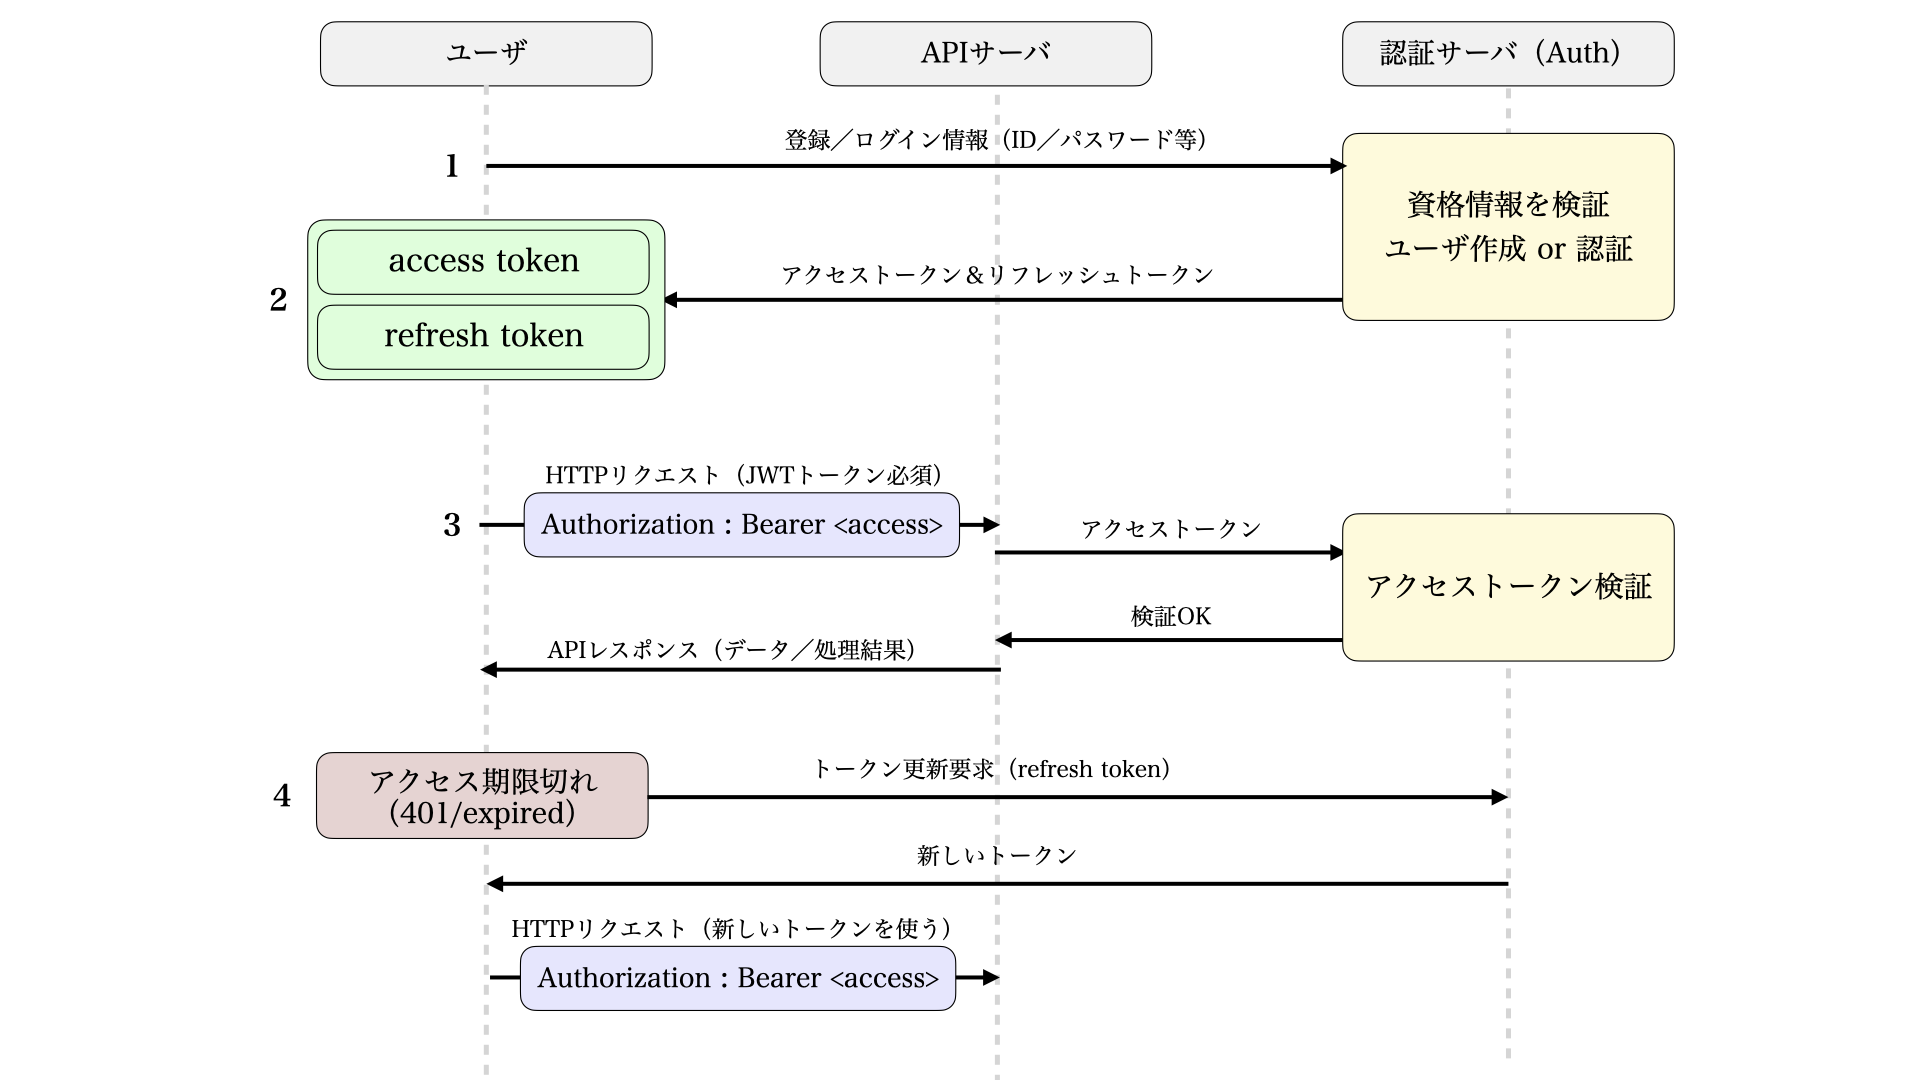
\includegraphics[scale = 0.3]{fig1.png}
\caption{JWT を用いた認証フロー(簡易図)}
\end{figure}


\subsection{ユーザー登録}

\begin{tcolorbox}[colback=blue!5,colframe=blue!50!black,title=エンドポイント]
\texttt{POST /api/v1/auth/sign-up}
\end{tcolorbox}

このエンドポイントでは、リクエストボディに含めた情報を持つユーザをデータベースに登録します。

\textbf{▼リクエストボディ}:
\begin{lstlisting}[style=json]
{
  "username": "string",        // 必須: ユーザー名
  "email": "user@example.com", // 必須: メールアドレス
  "password": "string",         // 必須: パスワード
  "profile_picture": "file",   // 任意: プロフィール画像
  "group": "string"            // 任意: グループ名
}
\end{lstlisting}

\textbf{▼レスポンス例} (201 Created):
\begin{lstlisting}[style=json]
{
  "message": "User registration successful"
}
\end{lstlisting}

\subsection{ログイン(JWTトークン取得)}

\begin{tcolorbox}[colback=blue!5,colframe=blue!50!black,title=エンドポイント]
\texttt{POST /api/v1/auth/jwt-token}
\end{tcolorbox}

このエンドポイントでは、リクエストボディのユーザ名、パスワードに対応する既存ユーザに対応するJWTトークンを取得します。

\textbf{▼リクエストボディ}:
\begin{lstlisting}[style=json]
{
  "username": "testuser",
  "password": "SecurePassword123!"
}
\end{lstlisting}

\textbf{▼レスポンス例} (200 OK):
\begin{lstlisting}[style=json]
{
  "access": "eyJ0eXAiOiJKV1QiLCJhbGciOiJIUzI1NiJ9...",
  "refresh": "eyJ0eXAiOiJKV1QiLCJhbGciOiJIUzI1NiJ9..."
}
\end{lstlisting}

\begin{tcolorbox}[colback=green!10,colframe=green!50!black,title=実装のヒント]
取得したaccess tokenは、以降のAPIリクエストで使用します。\\
ヘッダー形式: \texttt{Authorization: Bearer <access\_token>}
\end{tcolorbox}

\subsection{トークンのリフレッシュ}

\begin{tcolorbox}[colback=blue!5,colframe=blue!50!black,title=エンドポイント]
\texttt{POST /api/v1/auth/jwt-token/refresh}
\end{tcolorbox}

access tokenの有効期限が切れた場合、refresh tokenを使用して新しいaccess tokenを取得できます。

\textbf{▼リクエストボディ}:
\begin{lstlisting}[style=json]
{
  "refresh": "eyJ0eXAiOiJKV1QiLCJhbGciOiJIUzI1NiJ9..."
}
\end{lstlisting}

\subsection{ニーモニックフレーズの取得}
\textbf{ニーモニックフレーズ(Mnemonic Phrase)}とは、ウォレットの秘密鍵を人間が覚えやすい
12語や24語の単語列に変換したものです。  
これはウォレットを復元するための「根本的な情報」であり、他人に知られると資産を完全に奪われます。  
\textbf{パスワードを忘れても、ニーモニックさえあればウォレットを復元できますが、逆にニーモニックを失うと永久に資産へアクセスできなくなります。}

\begin{tcolorbox}[colback=red!10,colframe=red!50!black,title=セキュリティ警告]
ニーモニックフレーズは極めて重要な情報です。  
スクリーンショットやクラウド保存は避け、オフラインで安全に保管してください。  
他人に知られた場合、ウォレット資産は即座に盗まれる可能性があります。
\end{tcolorbox}

\begin{tcolorbox}[colback=blue!5,colframe=blue!50!black,title=エンドポイント]
\texttt{POST /api/v1/auth/mnemonic}
\end{tcolorbox}


\textbf{認証}: JWTトークン必須


\textbf{▼リクエストボディ}:
\begin{lstlisting}[style=json]
{
  "password": "YourCurrentPassword"
}
\end{lstlisting}

\section{BSV(Bitcoin SV)操作}

OrdinalXでは、BSVの送受信、残高確認などの操作を行うことができます。

\subsection{WhatsOnChain}
BSVの送受信は、すべて「トランザクション」としてブロックチェーンに書き込まれ(トランザクションID/\texttt{txid} が発行されます)、その記録はブロックチェーン・エクスプローラで誰でも確認できます。BSVでよく使われるエクスプローラの代表例が \textbf{WhatsOnChain(WOC)}です。API を叩いて返ってきた情報を確認するのはもちろん重要ですが、ときどき対象の \texttt{txid} を WOC でも検索し、伝播や承認数(confirmations)、入出力や手数料の内訳を合わせて見ておくと、状況判断がぐっと明確になります。

\begin{figure}[H]
\centering
% 左右で全く同じサイズの枠(幅・高さ)に収める
\begin{minipage}[t][0.28\textheight][c]{0.48\linewidth}
  \centering
  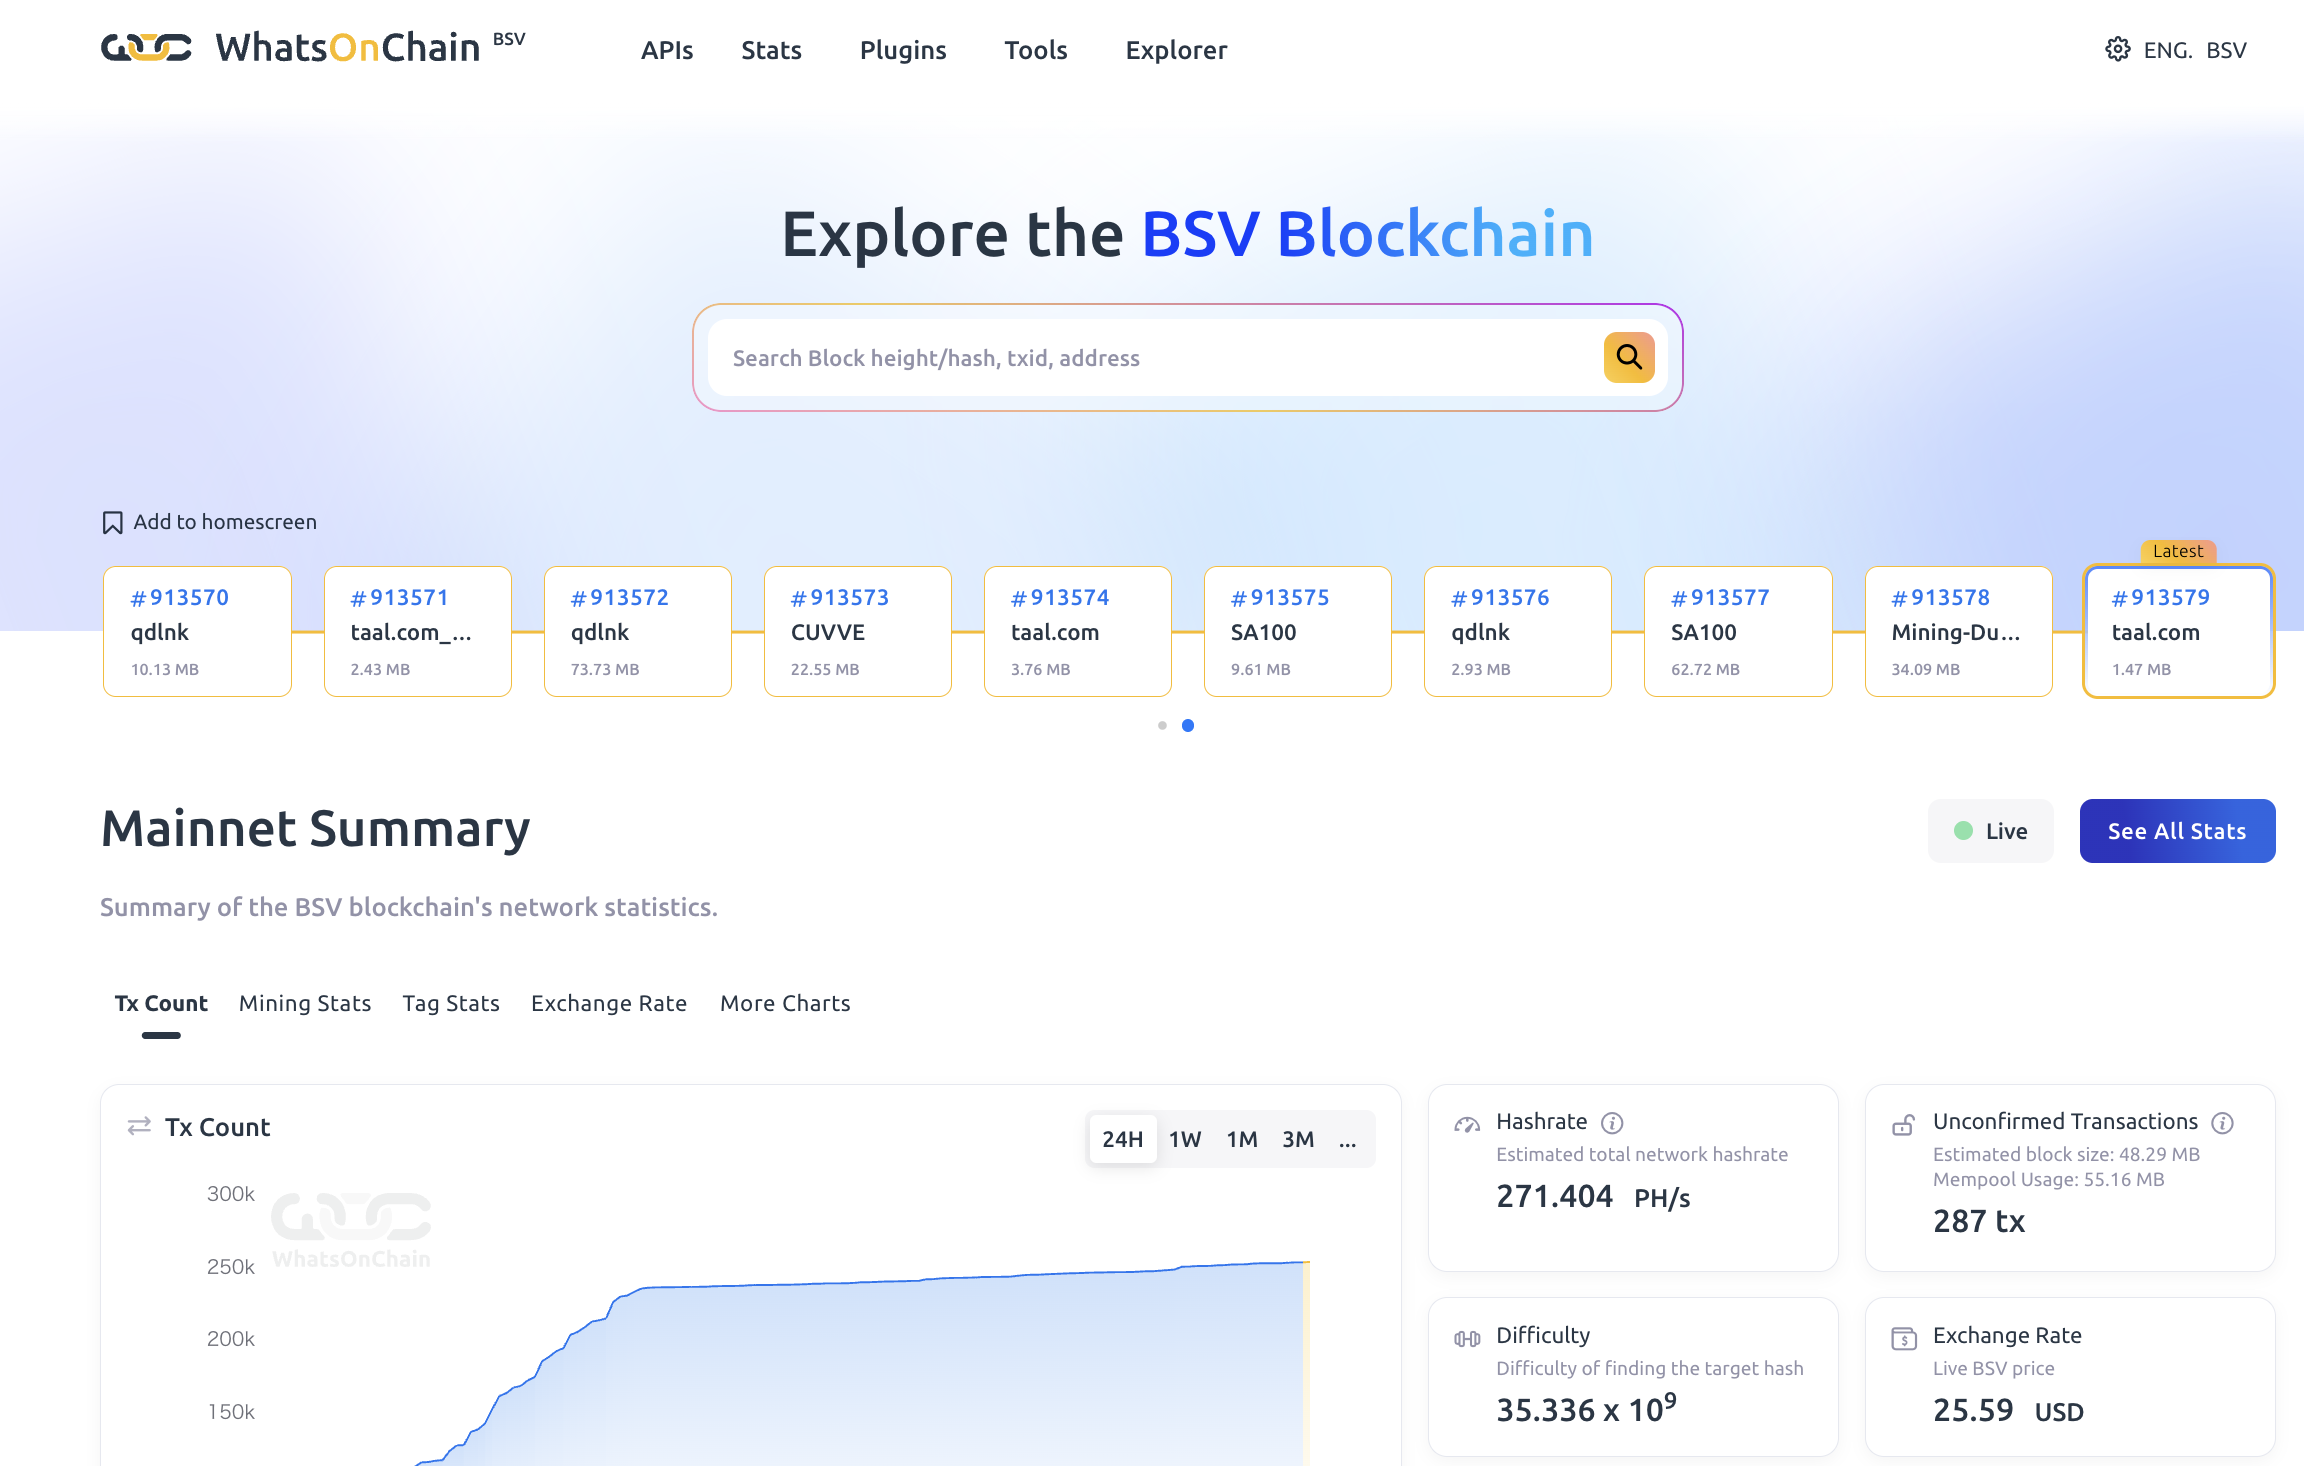
\includegraphics[width=\linewidth,height=0.28\textheight,keepaspectratio]{fig2.png}
\end{minipage}\hfill
\begin{minipage}[t][0.28\textheight][c]{0.48\linewidth}
  \centering
  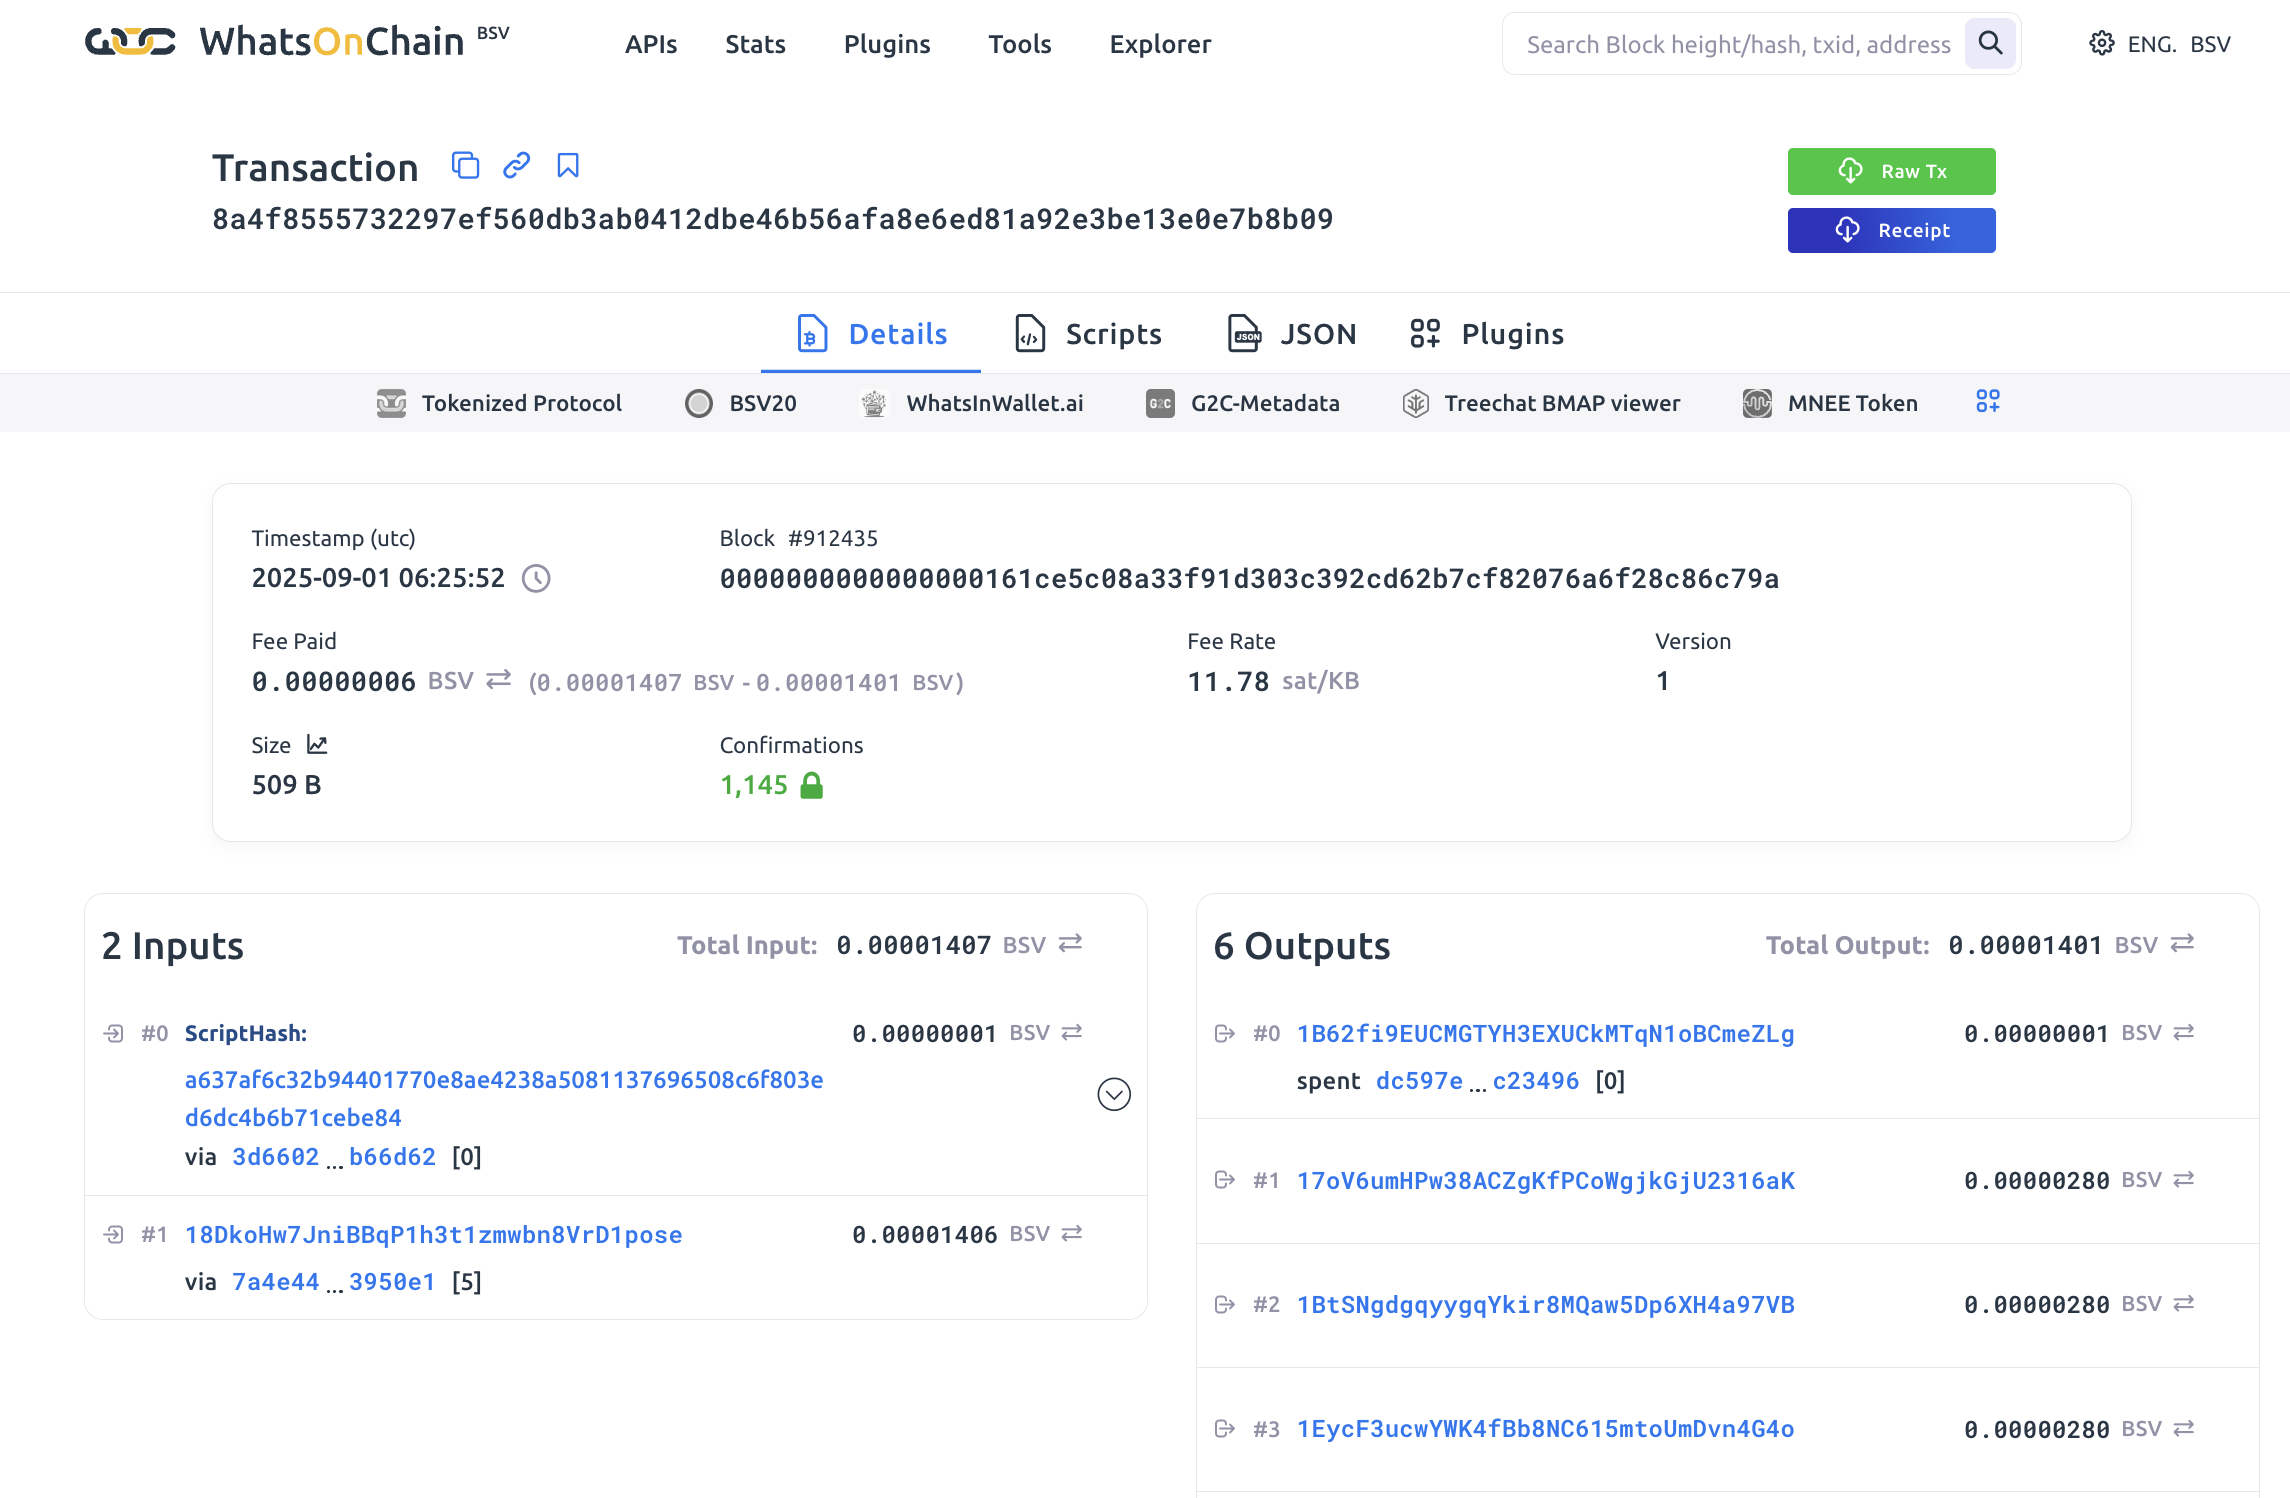
\includegraphics[width=\linewidth,height=0.28\textheight,keepaspectratio]{fig3.png}
\end{minipage}

% (任意)キャプション
\caption{WhatsOnChain}
\end{figure}



\subsection{残高確認}

誰のインプットにもなっていない自分宛てのアウトプットを\textbf{UTXO(Unspent transaction output)}といいます。BSVを誰かに送金するときは、自らに紐づいたUTXOからいくつかを選び、それを元手にして送金先宛のアウトプットを作成します。利用可能なUTXOの合計額を\textbf{残高(balance)}と呼びます。

\begin{tcolorbox}[colback=blue!5,colframe=blue!50!black,title=エンドポイント]
\texttt{GET /api/v1/user/wallet/balance}
\end{tcolorbox}

\textbf{認証}: JWTトークン必須

\textbf{▼レスポンス例}:
\begin{lstlisting}[style=json]
{
  "balance": 1000000  // satoshi単位
}
\end{lstlisting}

\begin{tcolorbox}[colback=yellow!10,colframe=orange!50!black,title=単位について]
BSVの残高はsatoshi単位で表示されます。\\
1 BSV = 100,000,000 satoshi
\end{tcolorbox}




\subsection{レガシーアドレスとpaymail}

レガシーアドレスは、ブロックチェーン上にそのまま記録される固定の受取先(長い文字列)です。Paymail(BSV alias とも)は \texttt{name@domain} のような人に伝えやすい別名で、送金時にウォレットが裏側で実際の受取先を毎回取得します。Paymailは再利用を避けやすく請求や共有に向き、レガシーは外部に依存せず機器間やオフライン運用に向きます。なお、WOCなどのエクスプローラで表示されるのは最終的なアドレスとトランザクションで、Paymail文字列自体は載りません。

\begin{tcolorbox}[colback=yellow!10,colframe=orange!50!black,title=OrdinalXはどちらも扱える]
OrdinalXでは、レガシーアドレス向け、paymail向け、どちらも扱うことができます。
\end{tcolorbox}

\subsection{BSV送金(Paymail宛)}

指定したPaymail宛に、指定した金額(\verb|amount_to_send|)を送金します。

\begin{tcolorbox}[colback=blue!5,colframe=blue!50!black,title=エンドポイント]
\texttt{POST /api/v1/bsv/paymail/send}
\end{tcolorbox}

\textbf{▼リクエストボディ}:
\begin{lstlisting}[style=json]
{
  "recipient_paymail": "user@example.com",
  "amount_satoshis": 10000  // 送金額(satoshi単位)
}
\end{lstlisting}

\textbf{▼レスポンス例}:
\begin{lstlisting}[style=json]
{
  "message": "Successfully Send BSV via Paymail",
  "transaction_id": "abc123def456...",
  "transaction_hex": "0100000001..."
}
\end{lstlisting}

\subsection{BSV送金(レガシーアドレス宛)}

指定したレガシーアドレス宛に、指定した金額(\verb|amount_to_send|)を送金します。

\begin{tcolorbox}[colback=blue!5,colframe=blue!50!black,title=エンドポイント]
\texttt{POST /api/v1/bsv/legacy-address/send}
\end{tcolorbox}

複数のアドレスへの一括送金にも対応しています。複数アドレスへの一括送信を行う際は、リクエストボディの\url{"recipient_address"}フィールドのリストに、送信先アドレスを追加します。全てのアドレスに同一金額(\url{"amount_to_send"})が送信されます。

\textbf{▼単一アドレスへの送金例}:
\begin{lstlisting}[style=json]
{
  "recipient_address": ["1KkyACvksLeTfw77h13Hv8NSpSUSx6QCPJ"],
  "amount_to_send": 1000
}
\end{lstlisting}

\textbf{▼複数アドレスへの送金例}:
\begin{lstlisting}[style=json]
{
  "recipient_address": [
    "1KkyACvksLeTfw77h13Hv8NSpSUSx6QCPJ",
    "1F49kAzgEbVR3z4eAbpRJbHWmaGXvK4asd"
  ],
  "amount_to_send": 500  // 各アドレスへの送金額
}
\end{lstlisting}

\subsection{レガシーアドレスの取得}

自分のウォレットのレガシーアドレスを取得します。

\begin{tcolorbox}[colback=blue!5,colframe=blue!50!black,title=エンドポイント]
\texttt{GET /api/v1/bsv/legacy-address}
\end{tcolorbox}

\textbf{認証}: JWTトークン必須

\textbf{▼レスポンス例}:
\begin{lstlisting}[style=json]
{
  "Address": ["1ABC...XYZ", "1DEF...UVW"]
}
\end{lstlisting}

\section{NFT(1SatOrdinals)操作}

\subsection{NFTの概要}
OrdinalXでは、BSVブロックチェーン上に\textbf{1SatOrdinals}という方法でNFT(Ordinals)を作成できます。

1SatOrdinalsとは、1 satoshiひとつひとつに通し番号(ordinal number)を振り、その 1 sat 自体にデータを刻む(inscribe)仕組みです。刻まれた 1satはNFT とみなされ、\textbf{所有権はその 1 sat を含む UTXO を誰が持っているか} で決まります。移転は通常の送金と同じく 1 sat を送るだけ。\textbf{ブロックチェーンを調べるだけでNFTは完全に追跡}できます。データはトランザクションに直接載るため改ざん不能で、手数料が低い BSV では画像・音声・文書なども実用サイズで \textbf{完全オンチェーン保存}が可能です。実運用では API が返す \texttt{txid} をエクスプローラ(WOC)で開けば、内容や移転履歴を自分の目で検証できます。


\begin{tcolorbox}[colback=red!10,colframe=red!50!black,title=NFTの公開は不可逆]
NFTの公開は不可逆なので機密や著作物の扱いには注意してください。
\end{tcolorbox}


\subsection{NFT作成(mint)}

NFT の \textbf{mint(ミント)}とは、新しく NFT を発行する行為を指します。OrdinalX では、ユーザーが指定したファイルやメタデータをトランザクションに含めて送信することで、その時点で 1 satoshi に刻まれた NFT が「誕生」します。ミントされた NFT は即座にオンチェーンに記録され、以降は \texttt{txid}(または \verb|nft_origin|) によって一意に識別できます。つまり、mint は「NFT を最初に生み出す操作」であり、ここから所有や送信といった後の利用が始まります。

\begin{tcolorbox}[colback=blue!5,colframe=blue!50!black,title=エンドポイント]
\texttt{POST /api/v1/nft/create}
\end{tcolorbox}

\textbf{リクエスト形式}: multipart/form-data

\textbf{パラメータ}:
\begin{itemize}
    \item \texttt{file} (必須): アップロードするファイル(最大25MB)
    \item \texttt{app} (必須): アプリケーション名
    \item \texttt{name} (必須): NFTの名前
    \item \texttt{recipient\_paymail} (任意): 受信者のPaymail(省略時は自分)
    \item \texttt{additional\_info} (任意): 追加メタデータ(JSON文字列)
\end{itemize}

\textbf{▼curlコマンド例}:
\begin{lstlisting}[style=bash]
curl -X POST https://akematsu.yenpoint.jp/api/v1/nft/create \
  -H "Authorization: Bearer YOUR_JWT_TOKEN" \
  -F "file=@/path/to/image.jpg" \
  -F "app=MyApp" \
  -F "name=My First NFT" \
  -F "recipient_paymail=friend@example.com"
\end{lstlisting}

\textbf{▼レスポンス例(mint成功)}:
\begin{lstlisting}[style=json]
{
  "message": "Successfully created NFT",
  "transaction_id": "a1b2c3d4e5f6...",
  "transaction_hex": "0100000001...",
  "nft_information": {
    "nft_id": 123,
    "nft_origin": "a1b2c3d4e5f6..._0",
    "original_file_name": "image.jpg",
    "content_type": "image/jpeg",
    "name": "My First NFT",
    "created_at": "2024-01-01T00:00:00Z"
  }
}
\end{lstlisting}

\begin{tcolorbox}[colback=green!10,colframe=green!50!black,title=実装のヒント]
\texttt{nft\_origin}は、NFTを一意に識別する重要な値です。送信や参照時に使用するので、必ず保存してください。

また、\texttt{nft\_origin}は、以下のような構造になっています。
\[
  \underbrace{\text{\texttt{52f…41d}}}_{\texttt{txid}}
  \text{\texttt{\_}}
  \underbrace{0}_{\substack{\text{vout}\\\text{番号}}}
\]

\end{tcolorbox}

\subsection{NFTの送信(移転)}

OrdinalXでは、NFTを簡単に誰かから誰かに移転できます。具体的には、データが刻み込まれた1satoshiをインプットとし、移転先のpaymailまたはレガシーアドレスをアウトプットとするトランザクションを発行します。

\subsection{NFT送信(Paymail宛)}
指定したpaymail宛に、\verb|nft_origin|に紐づいたNFTを送信します。
\begin{tcolorbox}[colback=blue!5,colframe=blue!50!black,title=エンドポイント]
\texttt{POST /api/v1/nft/paymail/send}
\end{tcolorbox}




\textbf{▼リクエストボディ}:
\begin{lstlisting}[style=json]
{
  "recipient_paymail": "friend@example.com",
  "nft_origin": "abc123..._0"
}
\end{lstlisting}

\subsection{NFT送信(レガシーアドレス宛)}

指定したレガシーアドレス宛に、\verb|nft_origin|に紐づいたNFTを送信します。

\begin{tcolorbox}[colback=blue!5,colframe=blue!50!black,title=エンドポイント]
\texttt{POST /api/v1/nft/legacy-address/send}
\end{tcolorbox}

\textbf{▼リクエストボディ}:
\begin{lstlisting}[style=json]
{
  "recipient_address": "1ABC...XYZ",
  "nft_origin": "abc123..._0"
}
\end{lstlisting}

\subsection{NFTデータの取得}

\begin{tcolorbox}[colback=blue!5,colframe=blue!50!black,title=エンドポイント]
\texttt{GET /api/v1/nft/data/\{nft\_origin\}}
\end{tcolorbox}

NFTの実際のデータ(画像など)を取得します。

\textbf{クエリパラメータ}:
\begin{itemize}
    \item \texttt{data\_format}: "base64"または"binary"(デフォルト: binary)
\end{itemize}

\subsection{保有NFT一覧の取得}

\begin{tcolorbox}[colback=blue!5,colframe=blue!50!black,title=エンドポイント]
\texttt{GET /api/v1/user/nfts/info}
\end{tcolorbox}

ユーザーが保有するすべてのNFTの情報を取得します。

\textbf{▼レスポンス例}:
\begin{lstlisting}[style=json]
[
  {
    "nft_id": 1,
    "nft_origin": "abc123..._0",
    "current_nft_location": "def456..._0",
    "original_file_name": "image.jpg",
    "content_type": "image/jpeg",
    "name": "My NFT",
    "metadata": {...},
    "created_at": "2024-01-01T00:00:00Z"
  }
]
\end{lstlisting}

\subsection{NFTのバーン(焼却)}

\begin{tcolorbox}[colback=red!10,colframe=red!50!black,title=警告]
NFTをバーンすると、そのNFTへのアクセス権を永久に失います。ただし、ブロックチェーン上のデータ自体は削除されません。
\end{tcolorbox}

\begin{tcolorbox}[colback=blue!5,colframe=blue!50!black,title=エンドポイント]
\texttt{POST /api/v1/nft/burn}
\end{tcolorbox}

\textbf{▼リクエストボディ}:
\begin{lstlisting}[style=json]
{
  "nft_origin": "abc123..._0"
}
\end{lstlisting}

\section{BEEF(Background Evaluation Extended Format)}

\subsection{BEEFとは}
BEEFは、BSVトランザクションの効率的な検証を可能にする形式です。
OrdinalXでは、1satoshi Ordinalsの送受信にBEEF形式を使用しています。

\subsection{BEEF形式でのNFT送信}

\begin{tcolorbox}[colback=blue!5,colframe=blue!50!black,title=エンドポイント]
\texttt{POST /api/v1/beef/1satord/paymail/send}
\end{tcolorbox}

このエンドポイントは、1satoshi OrdinalsをBEEF形式で送信する専用のものです。

\textbf{▼リクエストボディ}:
\begin{lstlisting}[style=json]
{
  "recipient_paymail": "friend@example.com",
  "nft_origin": "abc123..._0"
}
\end{lstlisting}

\section{Paymail機能}

\subsection{Paymailとは}
Paymailは、複雑なBSVアドレスを覚えやすいメールアドレス形式で表現する仕組みです。
例: \texttt{user@example.com}

\subsection{Paymail Discovery}

\begin{tcolorbox}[colback=blue!5,colframe=blue!50!black,title=エンドポイント]
\texttt{GET /.well-known/bsvalias}
\end{tcolorbox}

Paymailサービスの機能を確認するためのディスカバリーエンドポイントです。

\textbf{▼レスポンス例}:
\begin{lstlisting}[style=json]
{
  "bsvalias": "1.0",
  "capabilities": {
    "pki": "https://example.com/api/v1/bsvalias/pki/{alias}@{domain.tld}",
    "paymentDestination": "https://example.com/api/v1/bsvalias/address/{alias}@{domain.tld}"
  }
}
\end{lstlisting}

\subsection{公開鍵の取得}

\begin{tcolorbox}[colback=blue!5,colframe=blue!50!black,title=エンドポイント]
\texttt{GET /paymail/bsvalias/id/\{alias\_domain\}}
\end{tcolorbox}

指定したPaymailアドレスの公開鍵を取得します。

\subsection{プロフィール情報の取得}

\begin{tcolorbox}[colback=blue!5,colframe=blue!50!black,title=エンドポイント]
\texttt{GET /paymail/public-profile/\{alias\_domain\}}
\end{tcolorbox}

\textbf{▼レスポンス例}:
\begin{lstlisting}[style=json]
{
  "name": "John Doe",
  "avatar": "https://example.com/avatar.png"
}
\end{lstlisting}

\section{トランザクション管理}

\subsection{トランザクション履歴の取得}

\begin{tcolorbox}[colback=blue!5,colframe=blue!50!black,title=エンドポイント]
\texttt{GET /api/v1/user/transactions}
\end{tcolorbox}

\textbf{▼レスポンス例}:
\begin{lstlisting}[style=json]
[
  {
    "id": 1,
    "transaction_id": "abc123...",
    "fee": 100,
    "total_value": 10000,
    "transaction_type": 1,
    "status": "confirmed",
    "updated_at": "2024-01-01T00:00:00Z",
    "nfts": []
  }
]
\end{lstlisting}

\subsection{トランザクションタイプ}
\begin{itemize}
    \item タイプ1: 送金
    \item タイプ2: 受信
    \item タイプ3: NFT作成
    \item タイプ4: NFT送信
    \item タイプ5: NFT受信
    \item その他: システム定義のタイプ
\end{itemize}

\section{管理者機能}

\subsection{管理者権限について}
一部のエンドポイントは管理者権限が必要です。
これらは通常のユーザーアカウントではアクセスできません。

\subsection{ユーザーのNFT情報取得(管理者用)}

\begin{tcolorbox}[colback=blue!5,colframe=blue!50!black,title=エンドポイント]
\texttt{GET /api/v1/admin/nfts/info/\{username\}}
\end{tcolorbox}

指定したユーザーのNFT情報を管理者権限で取得します。

\subsection{NFTデータ取得(管理者用)}

\begin{tcolorbox}[colback=blue!5,colframe=blue!50!black,title=エンドポイント]
\texttt{GET /api/v1/admin/nft/data/\{nft\_origin\}}
\end{tcolorbox}

任意のNFTのデータを管理者権限で取得します。

\section{エラーハンドリング}

\subsection{標準的なHTTPステータスコード}

\begin{longtable}{|l|l|p{8cm}|}
\hline
\textbf{コード} & \textbf{状態} & \textbf{説明} \\
\hline
\endhead
200 & OK & リクエスト成功 \\
\hline
201 & Created & リソース作成成功 \\
\hline
400 & Bad Request & リクエスト形式エラー、バリデーションエラー \\
\hline
401 & Unauthorized & 認証失敗、トークン無効 \\
\hline
403 & Forbidden & 権限不足 \\
\hline
404 & Not Found & リソースが見つからない \\
\hline
500 & Internal Server Error & サーバー内部エラー \\
\hline
\end{longtable}

\subsection{エラーレスポンスの形式}

\begin{lstlisting}[style=json]
{
  "error": "Error message",
  "detail": "Detailed error description"  // 任意
}
\end{lstlisting}

\subsection{一般的なエラーとその対処法}

\subsubsection{認証エラー(401)}
\textbf{エラーメッセージ}: "Authentication credentials were not provided"

\textbf{対処法}:
\begin{itemize}
    \item Authorizationヘッダーが正しく設定されているか確認
    \item トークンの有効期限を確認
    \item 必要に応じてトークンをリフレッシュ
\end{itemize}

\subsubsection{バリデーションエラー(400)}
\textbf{エラーメッセージ}: "Invalid paymail format"

\textbf{対処法}:
\begin{itemize}
    \item Paymailの形式が正しいか確認(user@domain.com)
    \item 必須パラメータがすべて含まれているか確認
    \item データ型が正しいか確認
\end{itemize}


\section{よくある質問(FAQ)}

\subsection{一般的な質問}

\subsubsection{Q: 1satoshi Ordinalsとは何ですか?}
A: BSVの最小単位である1satoshiにデータを刻む技術です。これにより、極めて低コストでNFTを作成できます。
従来のNFTと異なり、トークン自体にデータが含まれているため、外部ストレージに依存しません。

\subsubsection{Q: Paymailアドレスはどのように取得できますか?}
A: OrdinalXでアカウントを作成すると、自動的にPaymailアドレスが割り当てられます。
形式は \texttt{username@domain.com} となります。

\subsubsection{Q: NFTの最大ファイルサイズは?}
A: 現在、25MBまでのファイルをアップロードできます。
これは画像、動画、ドキュメントなど、あらゆる形式のファイルに適用されます。

\subsubsection{Q: トランザクション手数料はどれくらいですか?}
A: BSVの手数料は非常に低く、通常1トランザクションあたり数satoshi(1円未満)です。
NFT作成時も同様に低コストで実行できます。

\subsection{技術的な質問}

\subsubsection{Q: JWTトークンの有効期限は?}
A: access tokenの有効期限は通常短く設定されています(数時間程度)。
refresh tokenを使用して定期的に更新してください。

\subsubsection{Q: 複数のNFTを一度に送信できますか?}
A: 現在のAPIでは、NFTは1つずつ送信する必要があります。
バッチ送信機能は将来的に実装される可能性があります。

\subsubsection{Q: バーンしたNFTは復元できますか?}
A: いいえ、一度バーンしたNFTへのアクセス権は永久に失われます。
ただし、ブロックチェーン上のデータ自体は残り続けます。

\subsubsection{Q: APIのレート制限はありますか?}
A: 具体的なレート制限は公開されていませんが、
過度なリクエストは制限される可能性があります。適切な間隔でリクエストを送信してください。

\subsection{トラブルシューティング}

\subsubsection{Q: "Invalid paymail format"エラーが出ます}
A: Paymailアドレスの形式を確認してください。
正しい形式: \texttt{user@example.com}
よくある間違い:
\begin{itemize}
    \item @マークが抜けている
    \item ドメイン部分が不完全
    \item 余分なスペースが含まれている
\end{itemize}

\subsubsection{Q: NFTが送信できません}
A: 以下を確認してください:
\begin{enumerate}
    \item NFTの所有権があるか(\texttt{nft\_origin}が正しいか)
    \item 受信者のPaymailまたはアドレスが正しいか
    \item 十分なBSV残高があるか(手数料分)
    \item 認証トークンが有効か
\end{enumerate}

\subsubsection{Q: トランザクションが確認されません}
A: BSVトランザクションは通常数秒で確認されますが、
ネットワークの混雑状況により遅延する場合があります。
トランザクションIDを使ってブロックエクスプローラーで状態を確認できます。

\section{サンプルコード}

\subsection{Python実装例}

\subsubsection{基本クラス}
\begin{lstlisting}[language=python, caption=Python実装]
import requests
from typing import Optional, Dict, Any

class OrdinalXClient:
    def __init__(self, base_url: str = 'https://akematsu.yenpoint.jp'):
        self.base_url = base_url
        self.token: Optional[str] = None
        self.refresh_token: Optional[str] = None
        self.session = requests.Session()
    
    def login(self, username: str, password: str) -> Dict[str, str]:
        """ユーザーログイン"""
        response = self.session.post(
            f'{self.base_url}/api/v1/auth/jwt-token',
            json={'username': username, 'password': password}
        )
        response.raise_for_status()
        
        data = response.json()
        self.token = data['access']
        self.refresh_token = data['refresh']
        self.session.headers.update({
            'Authorization': f'Bearer {self.token}'
        })
        
        return data
    
    def refresh_access_token(self) -> Dict[str, str]:
        """アクセストークンをリフレッシュ"""
        if not self.refresh_token:
            raise ValueError('No refresh token available')
        
        response = self.session.post(
            f'{self.base_url}/api/v1/auth/jwt-token/refresh',
            json={'refresh': self.refresh_token}
        )
        response.raise_for_status()
        
        data = response.json()
        self.token = data['access']
        self.session.headers.update({
            'Authorization': f'Bearer {self.token}'
        })
        
        return data
    
    def get_balance(self) -> Dict[str, Any]:
        """ウォレット残高取得"""
        response = self.session.get(
            f'{self.base_url}/api/v1/user/wallet/balance'
        )
        response.raise_for_status()
        return response.json()
    
    def send_bsv_paymail(
        self,
        recipient_paymail: str,
        amount_satoshis: int
    ) -> Dict[str, Any]:
        """Paymail宛BSV送金"""
        response = self.session.post(
            f'{self.base_url}/api/v1/bsv/paymail/send',
            json={
                'recipient_paymail': recipient_paymail,
                'amount_satoshis': amount_satoshis
            }
        )
        response.raise_for_status()
        return response.json()
    
    def create_nft(
        self,
        file_path: str,
        name: str,
        app: str,
        recipient_paymail: Optional[str] = None
    ) -> Dict[str, Any]:
        """NFT作成"""
        with open(file_path, 'rb') as f:
            files = {'file': f}
            data = {
                'name': name,
                'app': app
            }
            if recipient_paymail:
                data['recipient_paymail'] = recipient_paymail
            
            response = self.session.post(
                f'{self.base_url}/api/v1/nft/create',
                files=files,
                data=data
            )
        
        response.raise_for_status()
        return response.json()

# 使用例
if __name__ == '__main__':
    client = OrdinalXClient()
    
    # ログイン
    client.login('username', 'password')
    
    # 残高確認
    balance = client.get_balance()
    print(f"Balance: {balance['balance']} satoshis")
    
    # NFT作成
    nft_result = client.create_nft(
        file_path='image.jpg',
        name='My NFT',
        app='MyApp'
    )
    print(f"NFT created: {nft_result['nft_information']['nft_origin']}")
\end{lstlisting}

\section{付録}

\subsection{用語集}

\begin{description}
    \item[BSV (Bitcoin SV)] Bitcoin Satoshi Visionの略。スケーラビリティを重視したビットコインの実装。
    \item[Satoshi] BSVの最小単位。1 BSV = 100,000,000 satoshi。
    \item[Ordinals] ブロックチェーン上に直接データを記録するNFT技術。
    \item[Paymail] BSVアドレスをメールアドレス形式で表現する仕組み。
    \item[BEEF] Background Evaluation Extended Format。効率的なトランザクション検証形式。
    \item[JWT] JSON Web Token。認証用のトークン形式。
    \item[UTXO] Unspent Transaction Output。未使用のトランザクション出力。
    \item[Legacy Address] 従来形式のBSVアドレス(1で始まる)。
    \item[Mnemonic] ウォレット復元用の12-24単語のフレーズ。
    \item[Burn] NFTを焼却し、アクセス不可能にする操作。
\end{description}

\subsection{リンク集}

\begin{itemize}
    \item \textbf{API Base URL}: \url{https://akematsu.yenpoint.jp}
    \item \textbf{Swagger Documentation}: \url{https://akematsu.yenpoint.jp/?format=openapi}
    \item \textbf{BSV Block Explorer}: \url{https://whatsonchain.com}
\end{itemize}

\subsection{変更履歴}

\begin{itemize}
    \item \textbf{v1.0.0} - 初版リリース
    \item \textbf{v1.1.0} - BEEF形式のサポート追加
    \item \textbf{v1.2.0} - 25MBファイルアップロード対応
\end{itemize}

\end{document}
